\documentclass[preview]{standalone}
\usepackage{graphicx}
\usepackage{booktabs}
\usepackage{subcaption}
\begin{document}
	\begin{figure}
		\centering
		\begin{subfigure}{.5\textwidth}
			\centering
			\begin{tabular}{lll}
				\toprule
				$n$ & $V$ & $\approx V$ \\
				\midrule
				0 	& $1$ 						& $1$ \\
				1	& $2R$ 						& $2R$ \\
				2	& $\pi{}R^2$				& $3.14R^2$ \\
				3 	& $\frac{4}{3}\pi{}R^3$		& $4.19R^3$ \\
				4	& $\frac{\pi^2}{2}R^4$		& $4.94R^4$ \\
				5	& $\frac{8\pi^2}{15}R^5$	& $5.26R^5$ \\
				6 	& $\frac{\pi^3}{6}R^6$		& $5.17R^6$ \\
				7 	& $\frac{16\pi^3}{105}R^7$ 	& $4.73R^7$ \\
				8	& $\frac{\pi^4}{24}R^8$		&$4.06R^8$ \\
				\bottomrule
			\end{tabular}
		\end{subfigure}%
		\begin{subfigure}{.5\textwidth}
			\centering
			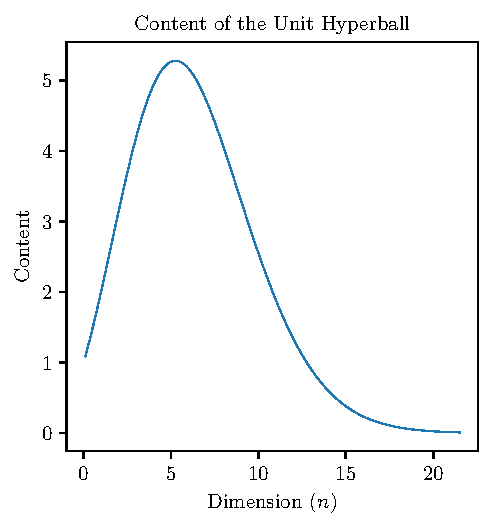
\includegraphics[width=\linewidth]{n-ball-graph-right.pdf}
		\end{subfigure}
	\end{figure}
\end{document}